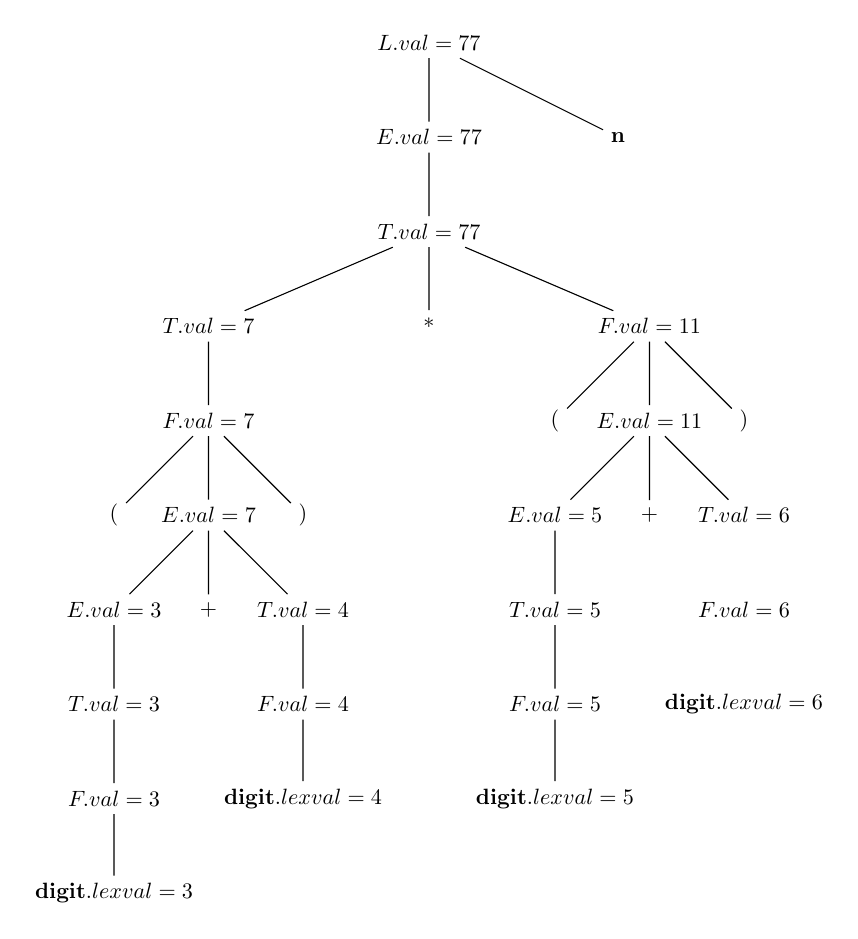
\begin{tikzpicture}[scale=0.8,every node/.style={scale=0.8}]
\node (v1) at (0,2.5) {$L.val=77$};
\node (v2) at (0,1) {$E.val=77$};
\node[font=\bfseries] (v3) at (3,1) {n};
\draw  (v1) edge (v2);
\draw  (v1) edge (v3);
\node (v4) at (0,-0.5) {$T.val=77$};
\draw  (v2) edge (v4);
\node (v6) at (0,-2) {*};
\node (v5) at (-3.5,-2) {$T.val=7$};
\node (v7) at (3.5,-2) {$F.val=11$};
\draw  (v4) edge (v5);
\draw  (v4) edge (v6);
\draw  (v4) edge (v7);
\node (v8) at (-3.5,-3.5) {$F.val=7$};
\draw  (v5) edge (v8);
\node (v10) at (-3.5,-5) {$E.val=7$};
\node (v9) at (-5,-5) {(};
\node (v11) at (-2,-5) {)};
\draw  (v8) edge (v9);
\draw  (v8) edge (v10);
\draw  (v8) edge (v11);
\node (v13) at (-3.5,-6.5) {+};
\node (v12) at (-5,-6.5) {$E.val=3$};
\node (v14) at (-2,-6.5) {$T.val=4$};
\draw  (v10) edge (v12);
\draw  (v10) edge (v13);
\draw  (v10) edge (v14);
\node (v15) at (-5,-8) {$T.val=3$};
\node (v16) at (-5,-9.5) {$F.val=3$};
\node (v17) at (-5,-11) {\textbf{digit}$.lexval=3$};
\draw  (v12) edge (v15);
\draw  (v15) edge (v16);
\draw  (v16) edge (v17);
\node (v18) at (-2,-8) {$F.val=4$};
\node (v19) at (-2,-9.5) {\textbf{digit}$.lexval=4$};
\draw  (v18) edge (v19);
\draw  (v14) edge (v18);
\node (v21) at (3.5,-3.5) {$E.val=11$};
\node (v20) at (2,-3.5) {(};
\node (v22) at (5,-3.5) {)};
\draw  (v7) edge (v20);
\draw  (v7) edge (v21);
\draw  (v7) edge (v22);
\node (v24) at (3.5,-5) {+};
\node (v23) at (2,-5) {$E.val=5$};
\node (v25) at (5,-5) {$T.val=6$};
\draw  (v21) edge (v23);
\draw  (v21) edge (v24);
\draw  (v21) edge (v25);
\node (v26) at (2,-6.5) {$T.val=5$};
\node (v27) at (2,-8) {$F.val=5$};
\node (v28) at (2,-9.5) {\textbf{digit}$.lexval=5$};
\draw  (v23) edge (v26);
\draw  (v26) edge (v27);
\draw  (v27) edge (v28);
\node at (5,-6.5) {$F.val=6$};
\node at (5,-8) {\textbf{digit}$.lexval=6$};
\end{tikzpicture}
